\section{Simulación}

Veremos una ejemplo para ver la capacidades de navindoor en un ejemplo real. Para ello previamente, hemos creado la planimtería del edifício de la facultad de ingeniería de Deusto, con ayuda de la interfaz gráfica \emph{navindoor}. Un vez creada podemos guardar esta en un archivo \emph{.mat} y utilizar las distintas funciones implentadas para la clase edifício. Un ejemplo muy util es utilizar la funcion plot sobre el objecto creado. Obtendrémos la figura \ref{UD_build}  
\begin{figure}\label{UD_build}
    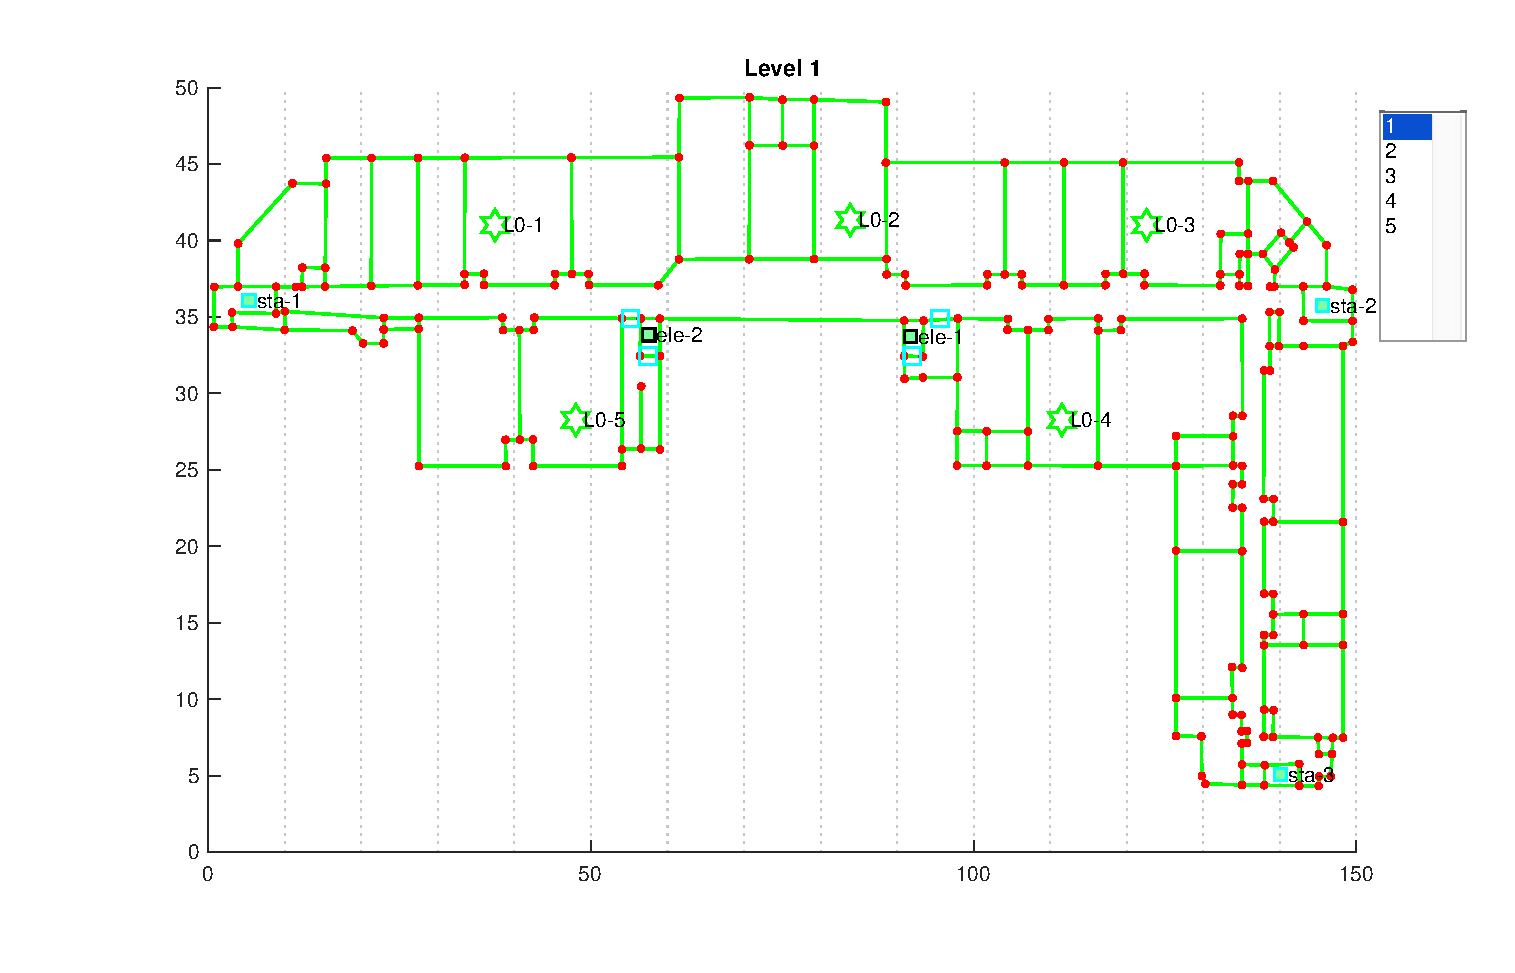
\includegraphics[width=1.0\columnwidth]{img/example/UD_build.eps}
    \caption[]{Visualización de la Facultad de ingeniería}
\end{figure}


